%% LyX 1.3 created this file.  For more info, see http://www.lyx.org/.
%% Do not edit unless you really know what you are doing.
\documentclass[english]{article}
\usepackage{float}
\usepackage{graphicx}

\makeatletter

%%%%%%%%%%%%%%%%%%%%%%%%%%%%%% LyX specific LaTeX commands.
%% Bold symbol macro for standard LaTeX users
\newcommand{\boldsymbol}[1]{\mbox{\boldmath $#1$}}


%%%%%%%%%%%%%%%%%%%%%%%%%%%%%% Textclass specific LaTeX commands.
 \newenvironment{lyxcode}
   {\begin{list}{}{
     \setlength{\rightmargin}{\leftmargin}
     \setlength{\listparindent}{0pt}% needed for AMS classes
     \raggedright
     \setlength{\itemsep}{0pt}
     \setlength{\parsep}{0pt}
     \normalfont\ttfamily}%
    \item[]}
   {\end{list}}

\usepackage{babel}
\makeatother
\begin{document}

\section{Introduction}

This report shows a comparison between the results of running several
different reinforcement learning algorithms and policies on the three
state problem, running on a simulated environment. All the implementation
is provided by libPG library. To make the comparison as fair as possible,
every algorithm uses a specifically tuned-up set of parameters values
($\kappa$, $\alpha$, $\lambda$ and $\epsilon$), which were found
by exhaustive search.

With softmax policy, the temperature decaying function used was $T(t)=\frac{1}{^{\left(1+\kappa t\right)2}}$
, where $t$ is the current time step and $\kappa$ is a constant.
Similarly, with $\epsilon$-greedy policy, the $\epsilon$ decaying
function used was $\epsilon(t)=\frac{1}{^{\left(1+\kappa t\right)2}}$.
In both cases the constant $\kappa$ defines how fast the used policy
becomes greedier with time, when selecting next actions. The others
parameters, $\alpha$ and $\lambda$, stands for step size and eligibility
traces, respectively.

The results of each algorithm and policy combination were averaged
over 100
 runs and the temporal difference discount used was $\gamma=0.6$
in all cases.


\section{The Three State Problem}

The three state simulator is a common place three-state POMDP employed
by Baxter et al and is implemented in libPG.


\section{Value Controllers}

The main idea of using SARSA and Q-Learning (as defined in sections
7.5 and 7.6 of \cite{rl}) to approach the three state problem is
to understand which policy evaluation approach (i.e. on-policy or
off-policy) performs better in this case. Also, since action selection
influences the results, we tried both softmax and $\epsilon$-greedy
policies. Below, it is presented the algorithms and the corresponding
resulting graphs.


\newpage
\subsection{SARSA($\lambda$) with Softmax Decaying Temperature Policy}

\begin{lyxcode}
double~discount~~=~0.4;

double~step\_size~=~0.001;

double~kapa~~~~~~=~1e-05;



Controller{*}~controller~=~new~SARSAController(

~~~~~~~~~~~~~~~~~~~~~~~~~new~NeuralNet(nnDims,~squash),

~~~~~~~~~~~~~~~(Policy{*})~new~SoftmaxPolicy(new~Temp(kapa)),~

~~~~~~~~~~~~~~~~~~~~~~~~~TD\_DISCOUNT);



OLPomdp{*}~learner~=~new~OLPomdp(controller,

~~~~~~~~~~~~~~~~~~~new~ThreeState(),~discount,~step\_size);
\end{lyxcode}
%
\begin{figure}[H]
\hfill{}\includegraphics[%
  scale=0.3]{Figures/SARSA_Lambda_Softmax_Decaying_Temperature.ps}\hfill{}


\caption{SARSA($\lambda$) with softmax policy (decaying temperature)}
\end{figure}



\newpage
\subsection{SARSA($\lambda$) with Constant $\epsilon$ $\epsilon$-Greedy Policy}

\begin{lyxcode}
double~discount~~=~0.5;

double~step\_size~=~0.001;

double~epsilon~~~=~0.01;



Controller{*}~controller~=~new~SARSAController(

~~~~~~~~~~~~~~~~~~~~~~~~~new~NeuralNet(nnDims,~squash)~

~~~~~~~~~~~~~~~(Policy{*})~new~eGreedyPolicy(epsilon),

~~~~~~~~~~~~~~~~~~~~~~~~~TD\_DISCOUNT);



OLPomdp{*}~learner~=~new~OLPomdp(controller,

~~~~~~~~~~~~~~~~~~~new~ThreeState(),~discount,~step\_size);
\end{lyxcode}
%
\begin{figure}[H]
\hfill{}\includegraphics[%
  scale=0.3]{Figures/SARSA_Lambda_e-Greedy_Constant_Epsilon.ps}\hfill{}


\caption{SARSA($\lambda$) with $\epsilon$-greedy policy (constant $\epsilon$)}
\end{figure}



\newpage
\subsection{SARSA($\lambda$) with Decaying $\epsilon$ $\epsilon$-Greedy Policy}

\begin{lyxcode}
double~discount~~=~0.7;

double~step\_size~=~0.001;

double~kapa~~~~~~=~0.001;



Controller{*}~controller~=~new~SARSAController(

~~~~~~~~~~~~~~~~~~~~~~~~~new~NeuralNet(nnDims,~squash),

~~~~~~~~~~~~~~~(Policy{*})~new~eGreedyPolicy(

~~~~~~~~~~~~~~~~~~~~~~~~~new~EpsilonDecay(kapa)),

~~~~~~~~~~~~~~~~~~~~~~~~~TD\_DISCOUNT);



OLPomdp{*}~learner~=~new~OLPomdp(controller,

~~~~~~~~~~~~~~~~~~~new~ThreeState(),~discount,~step\_size);
\end{lyxcode}
%
\begin{figure}[H]
\hfill{}\includegraphics[%
  scale=0.3]{Figures/SARSA_Lambda_e-Greedy_Decaying_Epsilon.ps}\hfill{}


\caption{SARSA($\lambda$) with $\epsilon$-greedy policy (decaying $\epsilon$)}
\end{figure}



\newpage
\subsection{Q-Learning($\lambda$) with Decaying Temperature Softmax Policy}

\begin{lyxcode}
double~discount~~=~0.4;

double~step\_size~=~0.001;

double~kapa~~~~~~=~1e-05;



Controller{*}~controller~=~new~QLearningController(

~~~~~~~~~~~~~~~~~~~~~~~~~new~NeuralNet(nnDims,~squash),

~~~~~~~~~~~~~~~(Policy{*})~new~SoftmaxPolicy(

~~~~~~~~~~~~~~~~~~~~~~~~~new~Temp(kapa)),

~~~~~~~~~~~~~~~~~~~~~~~~~TD\_DISCOUNT);



OLPomdp{*}~learner~=~new~OLPomdp(controller,

~~~~~~~~~~~~~~~~~~~new~ThreeState(),~discount,~step\_size);
\end{lyxcode}
%
\begin{figure}[H]
\hfill{}\includegraphics[%
  scale=0.3]{Figures/Q-Learning_Lambda_Softmax_Decaying_Temperature.ps}\hfill{}


\caption{Q-Learning($\lambda$) with softmax policy (decaying temperature)}
\end{figure}



\newpage
\subsection{Q-Learning($\lambda$) with Constant $\epsilon$ $\epsilon$-Greedy
Policy}

\begin{lyxcode}
double~discount~=~~0.5;

double~step\_size~=~0.001;

double~epsilon~=~~~0.01;



Controller{*}~controller~=~new~QLearningController(

~~~~~~~~~~~~~~~~~~~~~~~~~new~NeuralNet(nnDims,~squash),

~~~~~~~~~~~~~~~(Policy{*})~new~eGreedyPolicy(epsilon),

~~~~~~~~~~~~~~~~~~~~~~~~~TD\_DISCOUNT);



OLPomdp{*}~learner~=~new~OLPomdp(controller,

~~~~~~~~~~~~~~~~~~~new~ThreeState(),~discount,~step\_size);
\end{lyxcode}
%
\begin{figure}[H]
\hfill{}\includegraphics[%
  scale=0.3]{Figures/Q-Learning_Lambda_e-Greedy_Constant_Epsilon.ps}\hfill{}


\caption{Q-Learning($\lambda$) with $\epsilon$-greedy policy (constant $\epsilon$)}
\end{figure}



\newpage
\subsection{Q-Learning($\lambda$) with Decaying $\epsilon$ $\epsilon$-Greedy
Policy}

\begin{lyxcode}
double~discount~~=~0.4;

double~step\_size~=~0.001;

double~kapa~~~~~~=~0.001;



Controller{*}~controller~=~new~QLearningController(

~~~~~~~~~~~~~~~~~~~~~~~~~new~NeuralNet(nnDims,~squash),

~~~~~~~~~~~~~~~(Policy{*})~new~eGreedyPolicy(

~~~~~~~~~~~~~~~~~~~~~~~~~new~EpsilonDecay(kapa)),

~~~~~~~~~~~~~~~~~~~~~~~~~TD\_DISCOUNT);



OLPomdp{*}~learner~=~new~OLPomdp(controller,

~~~~~~~~~~~~~~~~~~~new~ThreeState(),~discount,~step\_size);
\end{lyxcode}
%
\begin{figure}[H]
\hfill{}\includegraphics[%
  scale=0.3]{Figures/Q-Learning_Lambda_e-Greedy_Decaying_Epsilon.ps}\hfill{}


\caption{Q-Learning($\lambda$) with $\epsilon$-greedy policy (decaying $\epsilon$)}
\end{figure}



\newpage
\subsection{Binary Controller}

\begin{lyxcode}
double~discount~~=~0.6;

double~step\_size~=~0.001;



Controller{*}~controller~=~new~BinaryController(

~~~~~~~~~~~~~~~~~~~~~~~~~new~NeuralNet(nnDims,~squash));



OLPomdp{*}~learner~=~new~OLPomdp(controller,

~~~~~~~~~~~~~~~~~~~new~ThreeState(),~discount,~step\_size);
\end{lyxcode}
%
\begin{figure}[H]
\hfill{}\includegraphics[%
  scale=0.3]{Figures/Binary_Controller.ps}\hfill{}


\caption{Binary controller}
\end{figure}



\section{Policy Gradient Controllers}

Natural Actor-Critics method (as defined in \cite{NAC}) was also
used in comparison with value methods.


\newpage
\subsection{NAC Transform}

\begin{lyxcode}
double~discount~=~~0.4;

double~step\_size~=~0.001;



Controller{*}~controller=~new~NACTransform(

~~~~~~~~~~~~~~~~~~~~~~~~new~BinaryController(

~~~~~~~~~~~~~~~~~~~~~~~~new~NeuralNetBatch(nnDims,~squash)),

~~~~~~~~~~~~~~~~~~~~~~~~TD\_DISCOUNT);



OLPomdp{*}~learner~=~new~OLPomdp(controller,

~~~~~~~~~~~~~~~~~~~new~ThreeState(),~discount,~step\_size);
\end{lyxcode}
%
\begin{figure}[H]
\hfill{}\includegraphics[%
  scale=0.3]{Figures/NAC_Transform.ps}\hfill{}


\caption{NAC Transform}
\end{figure}



\section{Conclusion}

Among value based algorithms, SARSA behaved slightly better than Q-Learning
when using the same policy. But, in both algorithms, $\epsilon$-greedy
with decaying $\epsilon$ performed better than softmax with decaying
temperature. The worst result was achieved with $\epsilon$-greedy
with constant $\epsilon$, as expected.

Natural Actor-Critics was the best of all methods by far, converging
very quickly to the optimum solution, being the most suited algorithm
for the three state problem.

\begin{thebibliography}{Peters, Vijayakumar and Schaal}
\bibitem[Sutton and Barto]{rl}Richard S. Sutton and Andrew G. Barto. \emph{Reinforcement Learning:
An Introduction}
\bibitem[Peters, Vijayakumar and Schaal]{NAC}Jan Peters, Sethu Vijayakumar, Stefan Schaal. \emph{Natural Actor-Critic}\end{thebibliography}

\end{document}
